% Copyright 2004 by Till Tantau <tantau@users.sourceforge.net>.
%
% In principle, this file can be redistributed and/or modified under
% the terms of the GNU Public License, version 2.
%
% However, this file is supposed to be a template to be modified
% for your own needs. For this reason, if you use this file as a
% template and not specifically distribute it as part of a another
% package/program, I grant the extra permission to freely copy and
% modify this file as you see fit and even to delete this copyright
% notice. 

\documentclass{beamer}

% There are many different themes available for Beamer. A comprehensive
% list with examples is given here:
% http://deic.uab.es/~iblanes/beamer_gallery/index_by_theme.html
% You can uncomment the themes below if you would like to use a different
% one:
%\usetheme{AnnArbor}
%\usetheme{Antibes}
%\usetheme{Bergen}
%\usetheme{Berkeley}
%\usetheme{Berlin}
%\usetheme{Boadilla}
%\usetheme{boxes}
%\usetheme{CambridgeUS}
%\usetheme{Copenhagen}
%\usetheme{Darmstadt}
%\usetheme{default}
%\usetheme{Frankfurt}
%\usetheme{Goettingen}
%\usetheme{Hannover}
%\usetheme{Ilmenau}
%\usetheme{JuanLesPins}
%\usetheme{Luebeck}
\usetheme{Madrid}
%\usetheme{Malmoe}
%\usetheme{Marburg}
%\usetheme{Montpellier}
%\usetheme{PaloAlto}
%\usetheme{Pittsburgh}
%\usetheme{Rochester}
%\usetheme{Singapore}
%\usetheme{Szeged}
%\usetheme{Warsaw}


% Customize Warsaw color 
\setbeamercolor*{palette primary}{use=structure,fg=white,bg=red!50!black}
\setbeamercolor*{palette secondary}{use=structure,fg=white,bg=red!60!black}
\setbeamercolor*{palette tertiary}{use=structure,fg=white,bg=red!70!black}

% Customize Warsaw block title and background colors
\setbeamercolor{block title}{bg=red!50!black,fg=white}


% List your packages here

\usepackage[colorinlistoftodos]{todonotes}
\usepackage{pgfgantt}

\title[Progress]{A Universal Platform for Building Energy Management}

% % A subtitle is optional and this may be deleted
% \subtitle{Product Proposal}

\author[B.~Lauer]{Brian~Lauer\\\and
Advisor: Dr. Suruz Miah}
% - Give the names in the same order as the appear in the paper.
% - Use the \inst{?} command only if the authors have different
%   affiliation.

\institute[Bradley University] % (optional, but mostly needed)
{
  Department of Electrical and Computer Engineering\\
  Bradley University\\
  1501 W. Bradley Avenue\\
  Peoria, IL, 61625, USA
}
% - Use the \inst command only if there are several affiliations.
% - Keep it simple, no one is interested in your street address.

\date[October~11,~2019]{Friday, October~11,~2019}
% - Either use conference name or its abbreviation.
% - Not really informative to the audience, more for people (including
%   yourself) who are reading the slides online

\logo{\hfill\href{http://www.bradley.edu}{\includegraphics[width=0.75cm]{figs/logoBU1-Print}}}  % place logo in every page 


\subject{Mobile Robot Localization}

% Let's get started
\begin{document}
\begin{frame}
  \titlepage
\end{frame}

\begin{frame}{Outline}
  \tableofcontents
  % You might wish to add the option [pausesections]
\end{frame}
%
\section{DC Motor Block Diagram}
\begin{frame}{DC Motor Block Diagram}
\begin{figure}
\centering
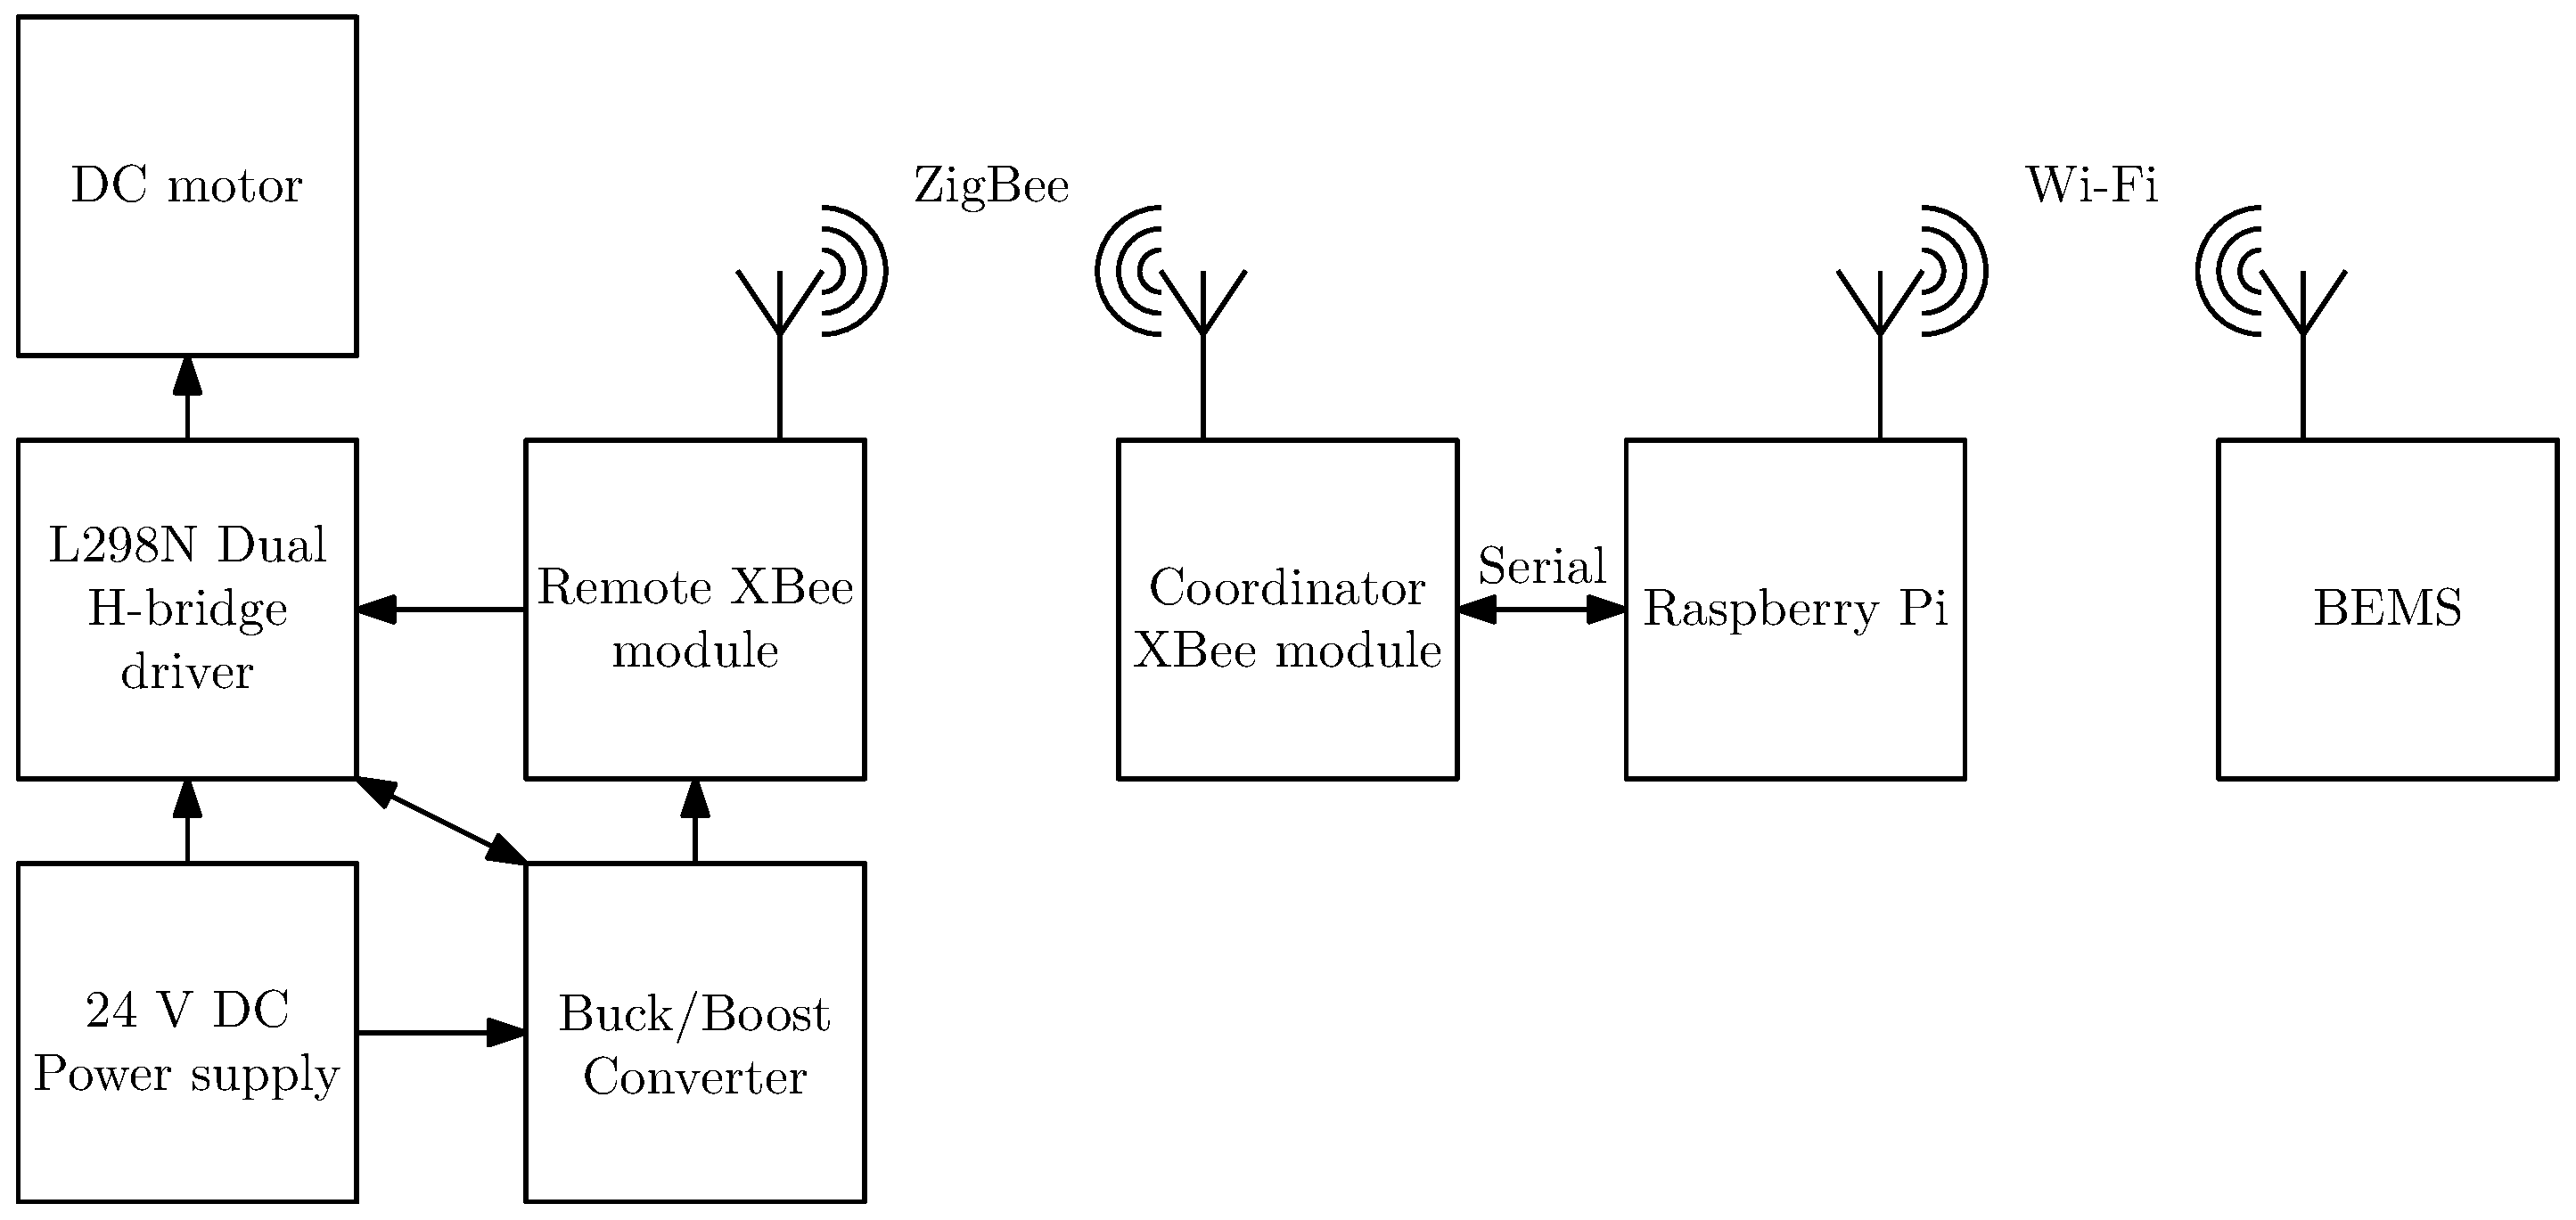
\includegraphics[scale=0.65]{figs/motorSetup}
\end{figure}
\end{frame}
%
\section{Current Work}
\begin{frame}{Current Work}
\begin{itemize}
\item Abandoned idea of Kill A Watt meter as the WeMo Insight Switch already measures power draw from the wall
\item Resarching new electrical load (IoT device)
\item Power demand ($W$, $kW$) will be monitored using the Switch
\end{itemize}
\end{frame}
%
\section{Current Schedule}
\begin{frame}{Current Schedule}
\begin{figure}[h]
%\begin{sidewaysfigure}
    \begin{ganttchart}[hgrid,
    vgrid={*4{black, dotted},*3{white},*1{black,
    dotted},*3{white},*1{black, dotted},*3{white}},
    group/.append style={draw=black, fill=yellow!50},
    group left shift = 0,
    group right shift = 0,
    y unit title=.8cm,
    %y unit chart=.8cm,
    milestone label font=\tiny,
    bar label font=\small, 
    group label font=\small,
    bar/.append style={draw=black,fill=blue},
    bar left shift= 0,
    bar right shift= 0,
    bar height = .2]{1}{16}
    \gantttitle{2019}{16}\\
    \gantttitle{Sep}{4}
    \gantttitle{Oct}{4}
    \gantttitle{Nov}{4}
    \gantttitle{Dec}{4}\\
    % \ganttgroup{DC motor speed control algorithm}{5}{8}\\
    \ganttgroup{Implement new device}{5}{12}\\
    \ganttbar{Research device}{5}{10}\\
    \ganttbar{Implemention in BEMOSS}{11}{12}\\
    \ganttgroup{DC motor speed control}{13}{15}\\
    \ganttbar{Research algorithm}{13}{15}
    \end{ganttchart}
\caption{Gantt chart for Fall 2019}
\label{gantt1}
\end{figure}
\end{frame}

\begin{frame}{Current Schedule}
\begin{figure}[h]
    \begin{ganttchart}[hgrid,
    vgrid={*4{black, dotted},*3{white},*1{black,
    dotted},*3{white},*1{black, dotted},*3{white},*1{black,dotted},*3{white}},
    group/.append style={draw=black, fill=yellow!50}, 
    group left shift = 0,
    group right shift = 0, 
    x unit=0.35cm,   
    y unit title=.8cm,
    %y unit chart=.8cm,
    milestone label font=\tiny,
    bar label font=\small, 
    group label font=\small,
    bar/.append style={draw = black, fill=blue},
    bar left shift= 0,
    bar right shift= 0,
    bar height = 0.2,
    bar incomplete/.append style={fill=red}]{1}{20}
    \gantttitle{2020}{20}\\
    \gantttitle{Jan}{4}
    \gantttitle{Feb}{4}
    \gantttitle{Mar}{4}
    \gantttitle{Apr}{4}
    \gantttitle{May}{4}\\
    \ganttgroup{DC motor speed control (cont.)}{2}{8}\\
    \ganttbar{Implementation in BEMOSS}{2}{8}\\
    \ganttgroup{Machine learning algorithm}{9}{18}\\
    \end{ganttchart}
\caption{Gantt chart for Spring 2020}
\label{gantt1}
\end{figure}
\end{frame}

% All of the following is optional and typically not needed. 
\appendix
\section<presentation>*{\appendixname}
\subsection<presentation>*{For Further Reading}

\begin{frame}[allowframebreaks]
  \frametitle<presentation>{For Further Reading}
    
  \begin{thebibliography}{10}
    
  \beamertemplatebookbibitems
  % Start with overview books.

  \bibitem{Author1990}
    A.~Author.
    \newblock {\em Handbook of Everything}.
    \newblock Some Press, 1990.
 
    
  \beamertemplatearticlebibitems
  % Followed by interesting articles. Keep the list short. 

  \bibitem{Someone2000}
    S.~Someone.
    \newblock On this and that.
    \newblock {\em Journal of This and That}, 2(1):50--100,
    2000.
  \end{thebibliography}
\end{frame}

\end{document}



%%% Local Variables:
%%% mode: latex
%%% TeX-master: t
%%% End:
